\documentclass[a4paper,12pt]{report}
\usepackage[T2A]{fontenc}
\usepackage[utf8]{inputenc}
\usepackage[english,russian]{babel}
\usepackage{graphicx}
\usepackage{wrapfig}
\usepackage{mathtext} 				% русские буквы в фомулах
\usepackage{amsmath,amsfonts,amssymb,amsthm,mathtools} % AMS
\usepackage{icomma} % "Умная" запятая: $0,2$ --- число, $0, 2$ --- перечисление
\usepackage{capt-of}
\usepackage{appendix}
\usepackage{multirow}
\usepackage{hyperref}
\usepackage{floatrow}
\usepackage[left=2cm,right=2cm,
    top=2cm,bottom=2cm,bindingoffset=0cm]{geometry}
\usepackage{multicol} % Несколько колонок
\usepackage{gensymb}
\title{Отчёт по лабораторной работе № 5.1.1. 

Экспериментальная проверка уравнения Эйнштейна для фотоэффекта и определение постоянной Планка.}
\author{Плюскова Н.А. Б04-004 }
\date{\today}
\begin{document}
\maketitle
\section*{1. Аннотация}
В данной работе была исследована зависимость фототока от величины задерживающего потенциала и частоты падающего излучения, а также вычислена величина постоянной Планка.


\section*{2. Теоретические сведения}

Фотоэффект --- явление испускания электронов фотокатодом, облучаемым светом,  Это явление хорошо объясняется фотонной теорией света. Взаимодействие монохроматического света с веществом можно описывать
	как взаимодействие с веществом частиц, называемых фотонами, которые обладают энергией $ \hbar \omega $ и импульсом $ \hbar\omega/c $. При столкновении фотона с электроном фотокатода энергия отона полностью передается электрону, и фотон прекращает свое существование. Энергетический баланс этого взаимодействия для вылетающих электронов
	описывается уравнением
	
	\begin{equation}\label{energy balance}
	\hbar \omega = E_{max} + W
	\end{equation}
	
	\begin{wrapfigure}{l}{0.4\linewidth}
		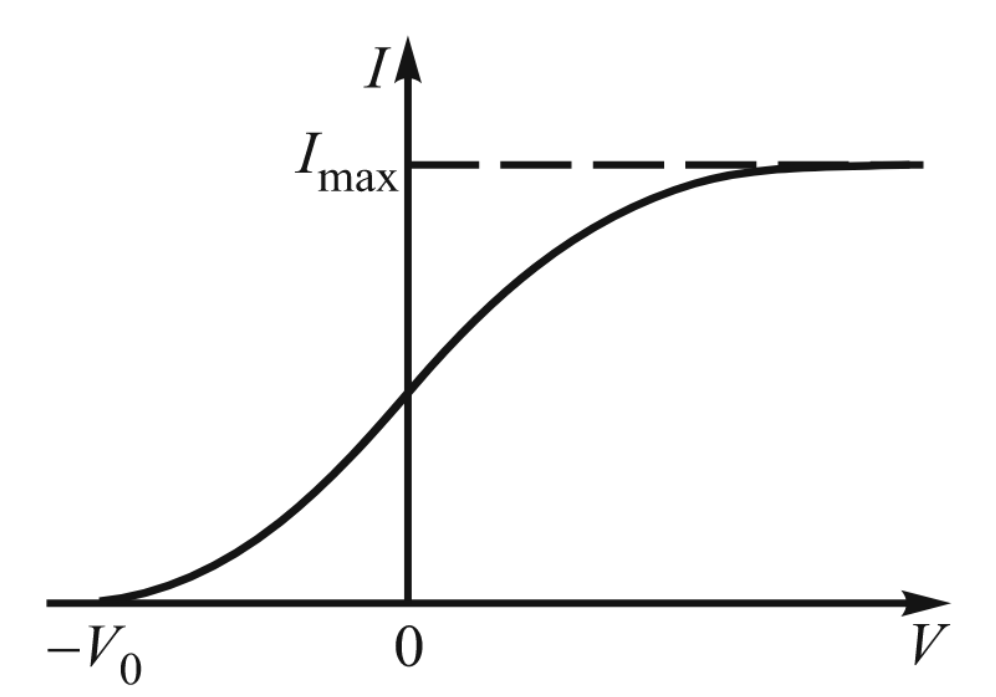
\includegraphics[width=\linewidth]{I_V.png}
		\caption{Зависимость фототока от напряжения на аноде фотоэлемента}
		\label{ris I(V)}
	\end{wrapfigure}
	
	Здесь $ E_{max} $ ---  максимальная кинетическая энергия электрона после выхода из фотокатода, $ W $ --- работа выхода электрона из катода. Реально энергетический спектр вылетевших из фотокатода электронов непрерывен --- он простирается от нуля до $ E_{max} $. 
	
	Для измерения энергии вылетевших фотоэлектронов вблизи фотокатода
	обычно располагается второй электрод
	(анод), на который подается задерживающий ($ V < 0 $) или ускоряющий ($ V >
	0 $) потенциал. При достаточно больших
	ускоряющих напряжениях фототок достигает насыщения (рис. \ref{ris I(V)}): все испущенные электроны попадают на анод.
	
	При задерживающих потенциалах на анод попадают лишь электроны,
	обладающие достаточно большой кинетической энергией, в то время
	как медленно движущиеся электроны заворачиваются полем и возвращаются на катод. При некотором значении $ V = -V_0 $ (потенциал запирания) даже наиболее быстрые фотоэлектроны не могут достичь
	анода.
	Максимальная кинетическая энергия $ E_{max} $ электронов связана с
	запирающим потенциалом $ V_0 $ очевидным соотношением $ E_{max} = eV_0 $. Тогда \eqref{energy balance} примет вид, называемый уравнением Эйнштейна:
	
	\begin{equation}\label{Einsteain}
	eV_0 = \hbar\omega - W 
	\end{equation}
	
	Чтобы определить величину запирающего
	напряжения, нам надо правильно экстраполировать получаемую токовую зависимость к нулю, т. е. определить, какова функциональная
	зависимость $ I(V) $. Расчет для простейшей геометрии --- плоский катод, освещаемый светом, и параллельный ему анод --- приводит к зависимости
	
	\begin{equation}\label{sqrt I = V}
	\sqrt{I} \propto V_0 - V
	\end{equation}
	
	т. е. корень квадратный из фототока линейно
	зависит от запирающего напряжения. Эта зависимость хорошо описывает экспериментальные данные.
	
	В работе изучается зависимость фототока из фотоэлемента от величины задерживающего потенциала $ V $ для различных частот света $ \omega $, лежащих в видимой области спектра. С целью экспериментальной
	проверки уравнения Эйнштейна определяются потенциалы запирания
	$ V_0 $ при разных частотах света и строится зависимость $ V_0(\omega) $, которая, как это следует из \eqref{Einsteain}, должна иметь вид
	

 	\begin{equation}\label{V(w)}
	V_0 (\omega) = \dfrac{\hbar\omega - W}{e}
	\end{equation}
 
	Потенциал запирания $ V_0 $ для любого катода линейно зависит от
	частоты света $ \omega $. По наклону прямой на графике $ V_0(\omega) $ (рис. \ref{ris V(w)}) можно определить постоянную Планка:
	
	\begin{equation}\label{dV/dw}
	\dfrac{dV_0}{d\omega} = \dfrac{\hbar}{e}
	\end{equation}


\begin{figure}[H]
\centering
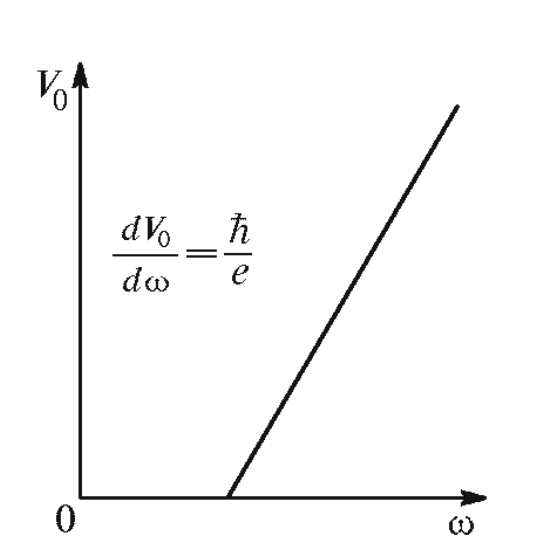
\includegraphics[width=0.4\linewidth]{V_w.png}
\caption{Зависимость запирающего потенциала от частоты света}
\label{ris V(w)}
\end{figure}

 
Как показывает формула \eqref{dV/dw}, угол наклона прямой $ V_0(\omega) $ не зависит от рода вещества, из которого изготовлен фотокатод. От рода вещества, однако, зависит величина фототока, работа выхода $ W $ и форма кривой $ I(V) $ (рис. \ref{ris I(V)}). Все это определяет выбор пригодных для
	опыта катодов.

 
\section*{3. Экспериментальная установка}
В данной работе для исследования зависимости фототока от величины запирающего потенциала используется монохроматор УМ-2. 

Свет от источника $S$ (электрическая лампа накаливания) с помощью конденсатора фокусируется на входную щель призменного монохроматора УМ-2, выделяющего узкий спектральный интервал, и попадает на катод фотоэлемента Ф-25. В качестве катода в данном элементе используется $Na_{2}KSb(Cs)$ покрытие.

\begin{figure}[H]
\centering
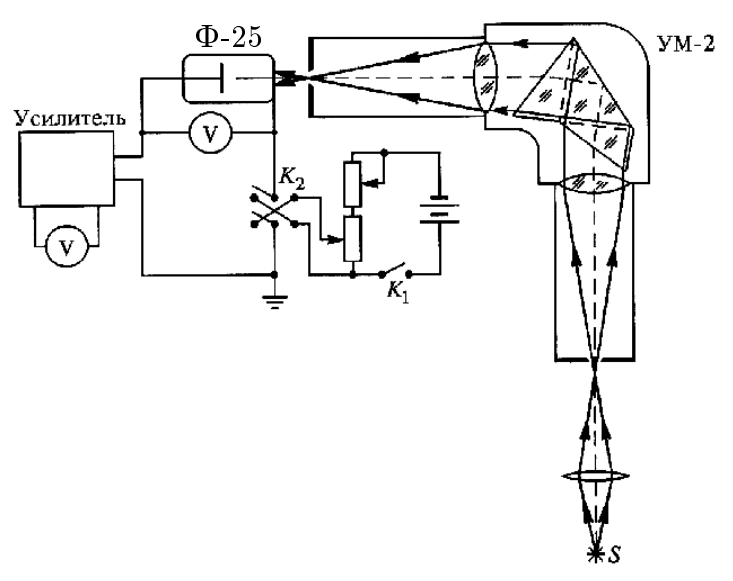
\includegraphics[width=0.6\linewidth]{ustanovka.png}
\caption{Схема экспериментальной установки}
\end{figure}
	
\section*{4. Ход работы}
\subsection*{4.1 Градуировка монохроматора}
Проградуируем барабан монохроматора по спектру неоновой лампы:
\begin{table}[H]
\begin{tabular}{|c|c|c|}
\hline
$\Theta, ^{o}$ & $\sigma_{\Theta}, ^{o}$     & $\lambda$, $A^{o}$ \\ \hline
3022     & \multirow{13}{*}{1} & 7032                         \\ \cline{1-1} \cline{3-3} 
2992     &                     & 6929                         \\ \cline{1-1} \cline{3-3} 
2928     &                     & 6717                         \\ \cline{1-1} \cline{3-3} 
2912     &                     & 6678                         \\ \cline{1-1} \cline{3-3} 
2889     &                     & 6599                         \\ \cline{1-1} \cline{3-3} 
2862     &                     & 6533                         \\ \cline{1-1} \cline{3-3} 
2856     &                     & 6507                         \\ \cline{1-1} \cline{3-3} 
2820     &                     & 6402                         \\ \cline{1-1} \cline{3-3} 
2811     &                     & 6383                         \\ \cline{1-1} \cline{3-3} 
2790     &                     & 6334                         \\ \cline{1-1} \cline{3-3} 
2778     &                     & 6305                         \\ \cline{1-1} \cline{3-3} 
2765     &                     & 6267                         \\ \cline{1-1} \cline{3-3} 
2747     &                     & 6217                         \\ \hline
\end{tabular}
\hspace{1.5 cm}
\begin{tabular}{|c|c|c|}
\hline
$\Theta, ^{o}$ & $\sigma_{\Theta}, ^{o}$     & $\lambda$, $A^{o}$  \\ \hline
2724     & \multirow{12}{*}{1} & 6164                         \\ \cline{1-1} \cline{3-3} 
2714     &                     & 6143                         \\ \cline{1-1} \cline{3-3} 
2692     &                     & 6096                         \\ \cline{1-1} \cline{3-3} 
2684     &                     & 6074                         \\ \cline{1-1} \cline{3-3} 
2666     &                     & 6030                         \\ \cline{1-1} \cline{3-3} 
2640     &                     & 5976                         \\ \cline{1-1} \cline{3-3} 
2626     &                     & 5945                         \\ \cline{1-1} \cline{3-3} 
2595     &                     & 5882                         \\ \cline{1-1} \cline{3-3} 
2580     &                     & 5852                         \\ \cline{1-1} \cline{3-3} 
2318     &                     & 5401                         \\ \cline{1-1} \cline{3-3} 
2282     &                     & 5341                         \\ \cline{1-1} \cline{3-3} 
2271     &                     & 5331                         \\ \hline
\end{tabular}
\caption{Градуировка монохроматора}
\end{table}

Построим соответствующий график:

\begin{figure}[H]
\centering
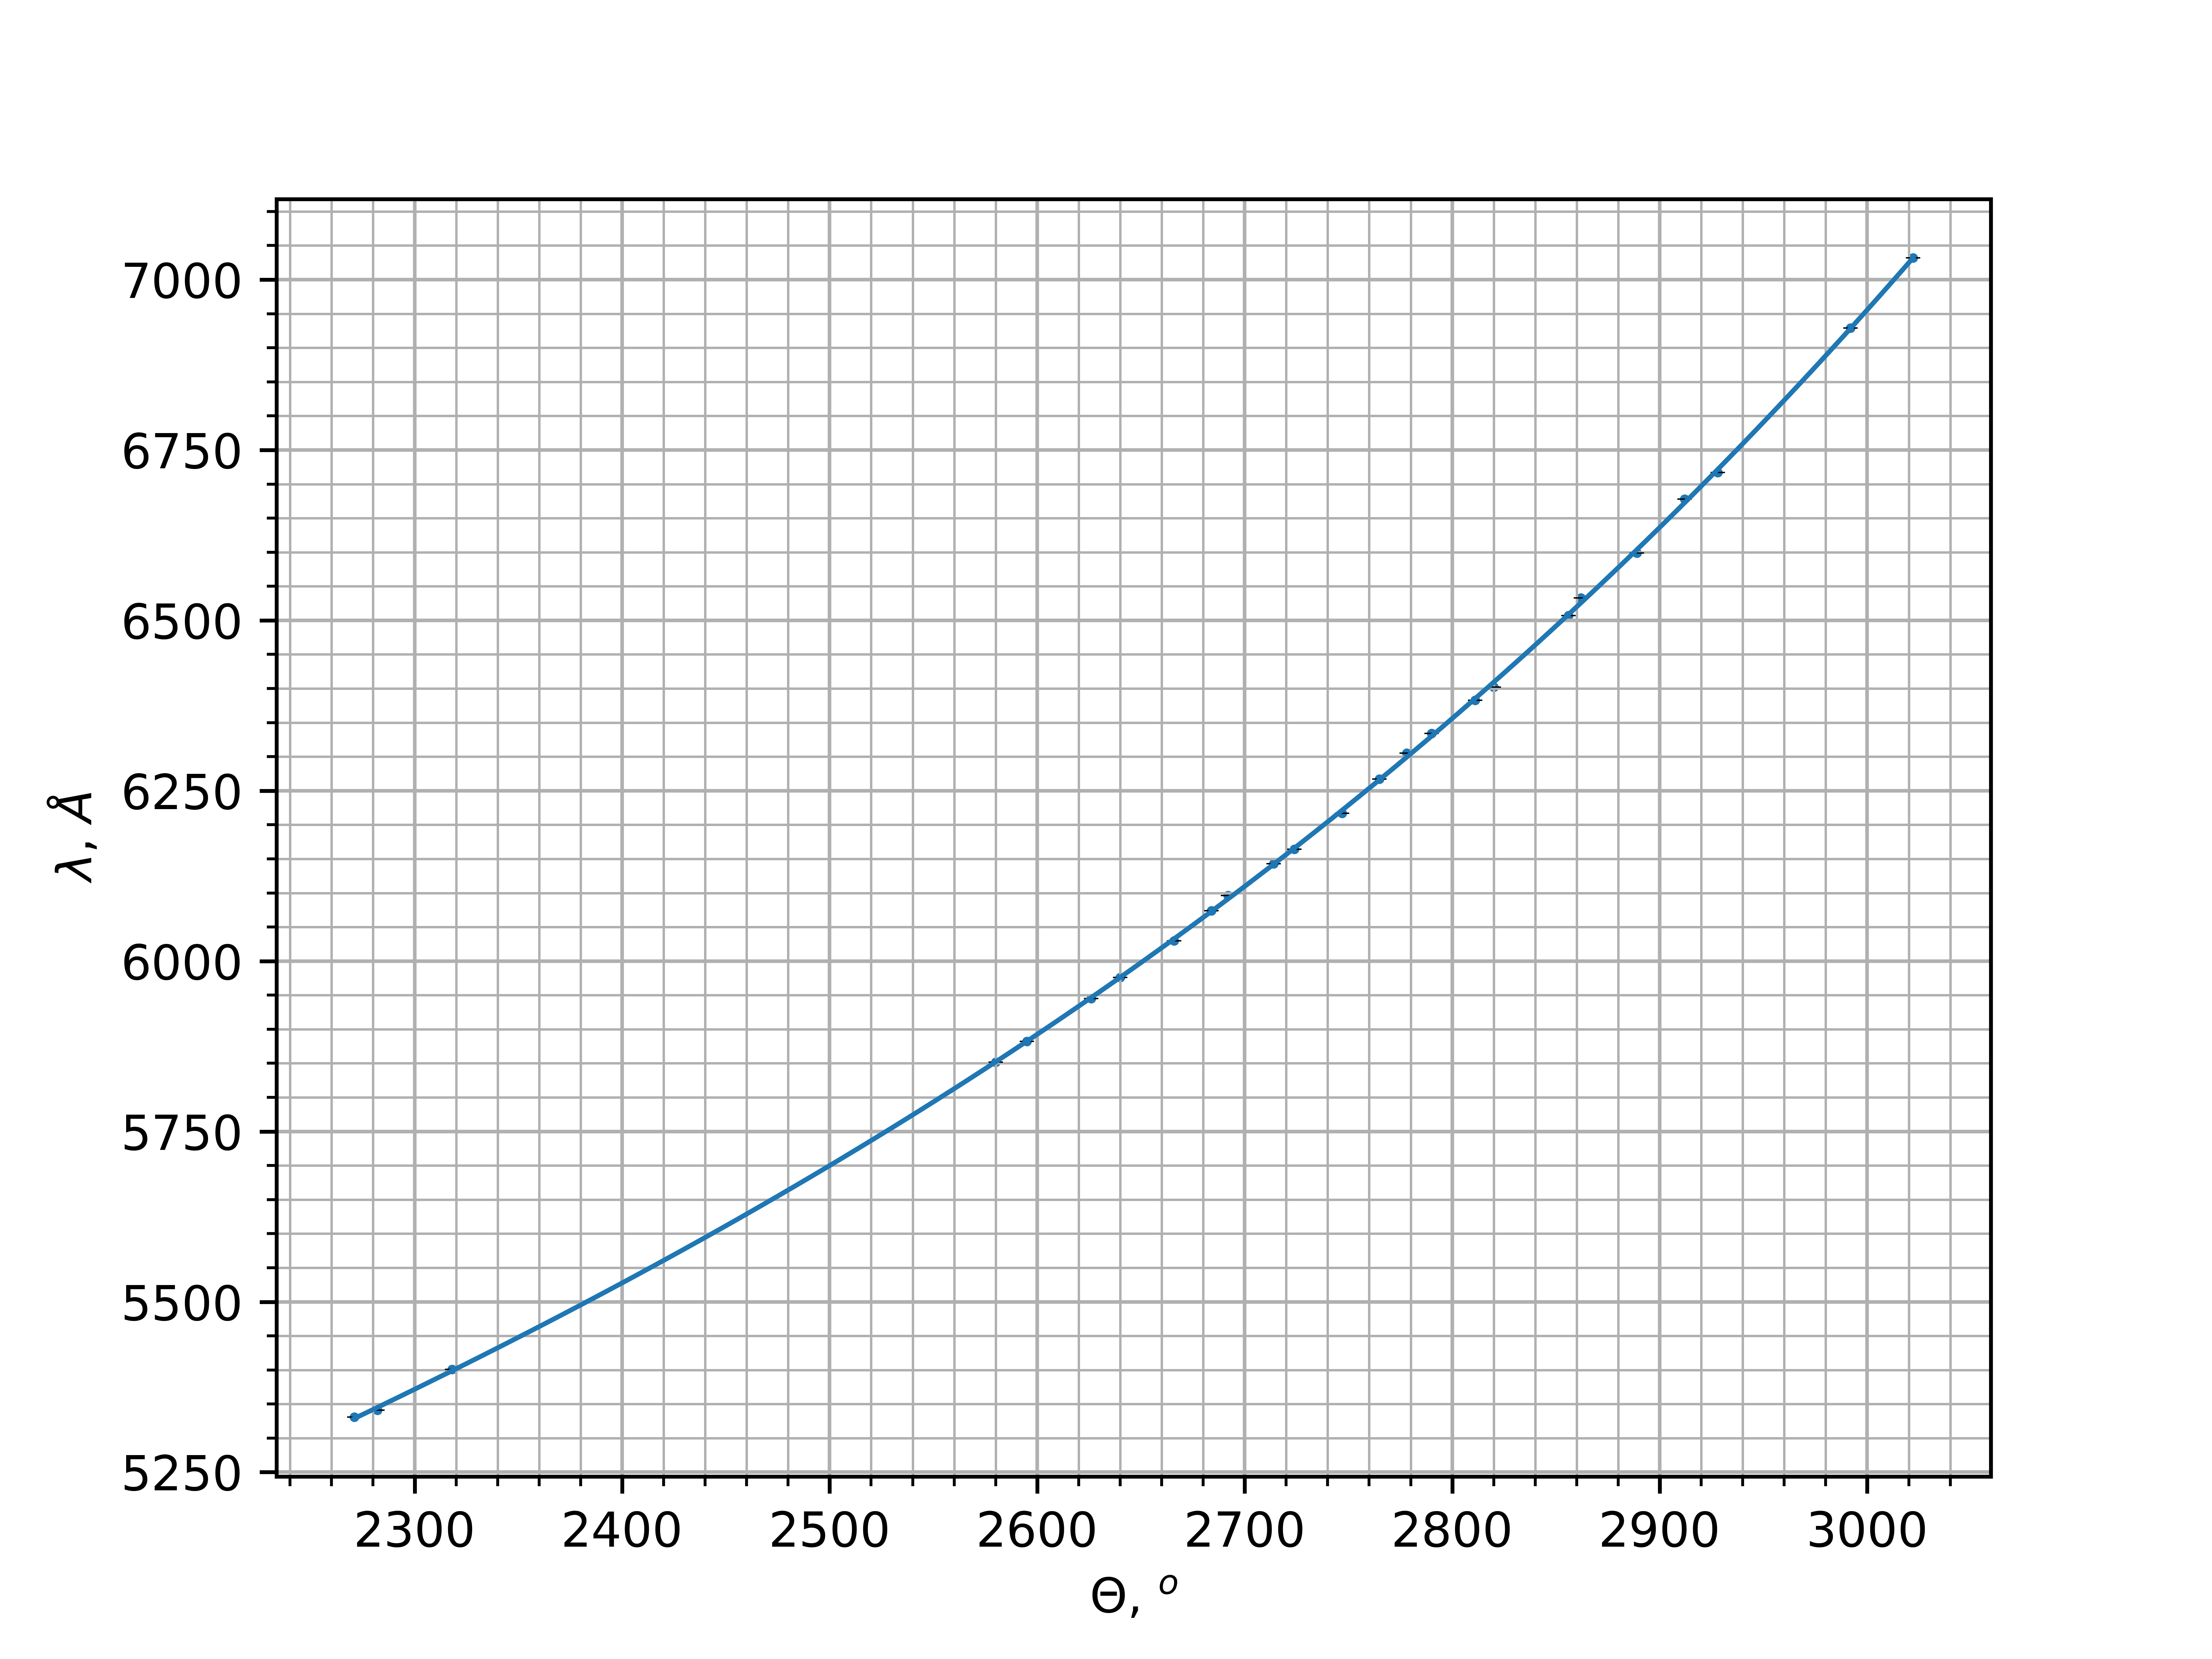
\includegraphics[width=0.7\linewidth]{grad.png}
\caption{Градуировочная кривая $\lambda(\theta)$}
\label{ris grad}
\end{figure}

Получаем нелинейную градуировку, которую аппроксимируем полиномом 5 степени:
\begin{equation*}
    y = A + Bx + Cx^2 + Dx^3 + Ex^4
\end{equation*}
\begin{center}
$A = -326,4; \ B = 4,83;\ C = -1,18 \cdot 10^{-3};\ D = -1,24 \cdot 10^{-7}; \ E = 8,33 \cdot 10^{-11}$    
\end{center}

\subsection*{4.2 Исследование зависимости фототока от величины запирающего потенциала}

Проведем 6 серий измерений зависимости фототока от напряжения для разных длин волн падающего света. На барабане монохроматора установим нужные нам длины волн, которые сможем определить с помощью градуировочного графика (таблица измерений представлена в Приложении)

Построим зависимость $V_{I}(V)$:

	\begin{figure}[H]
		\centering
		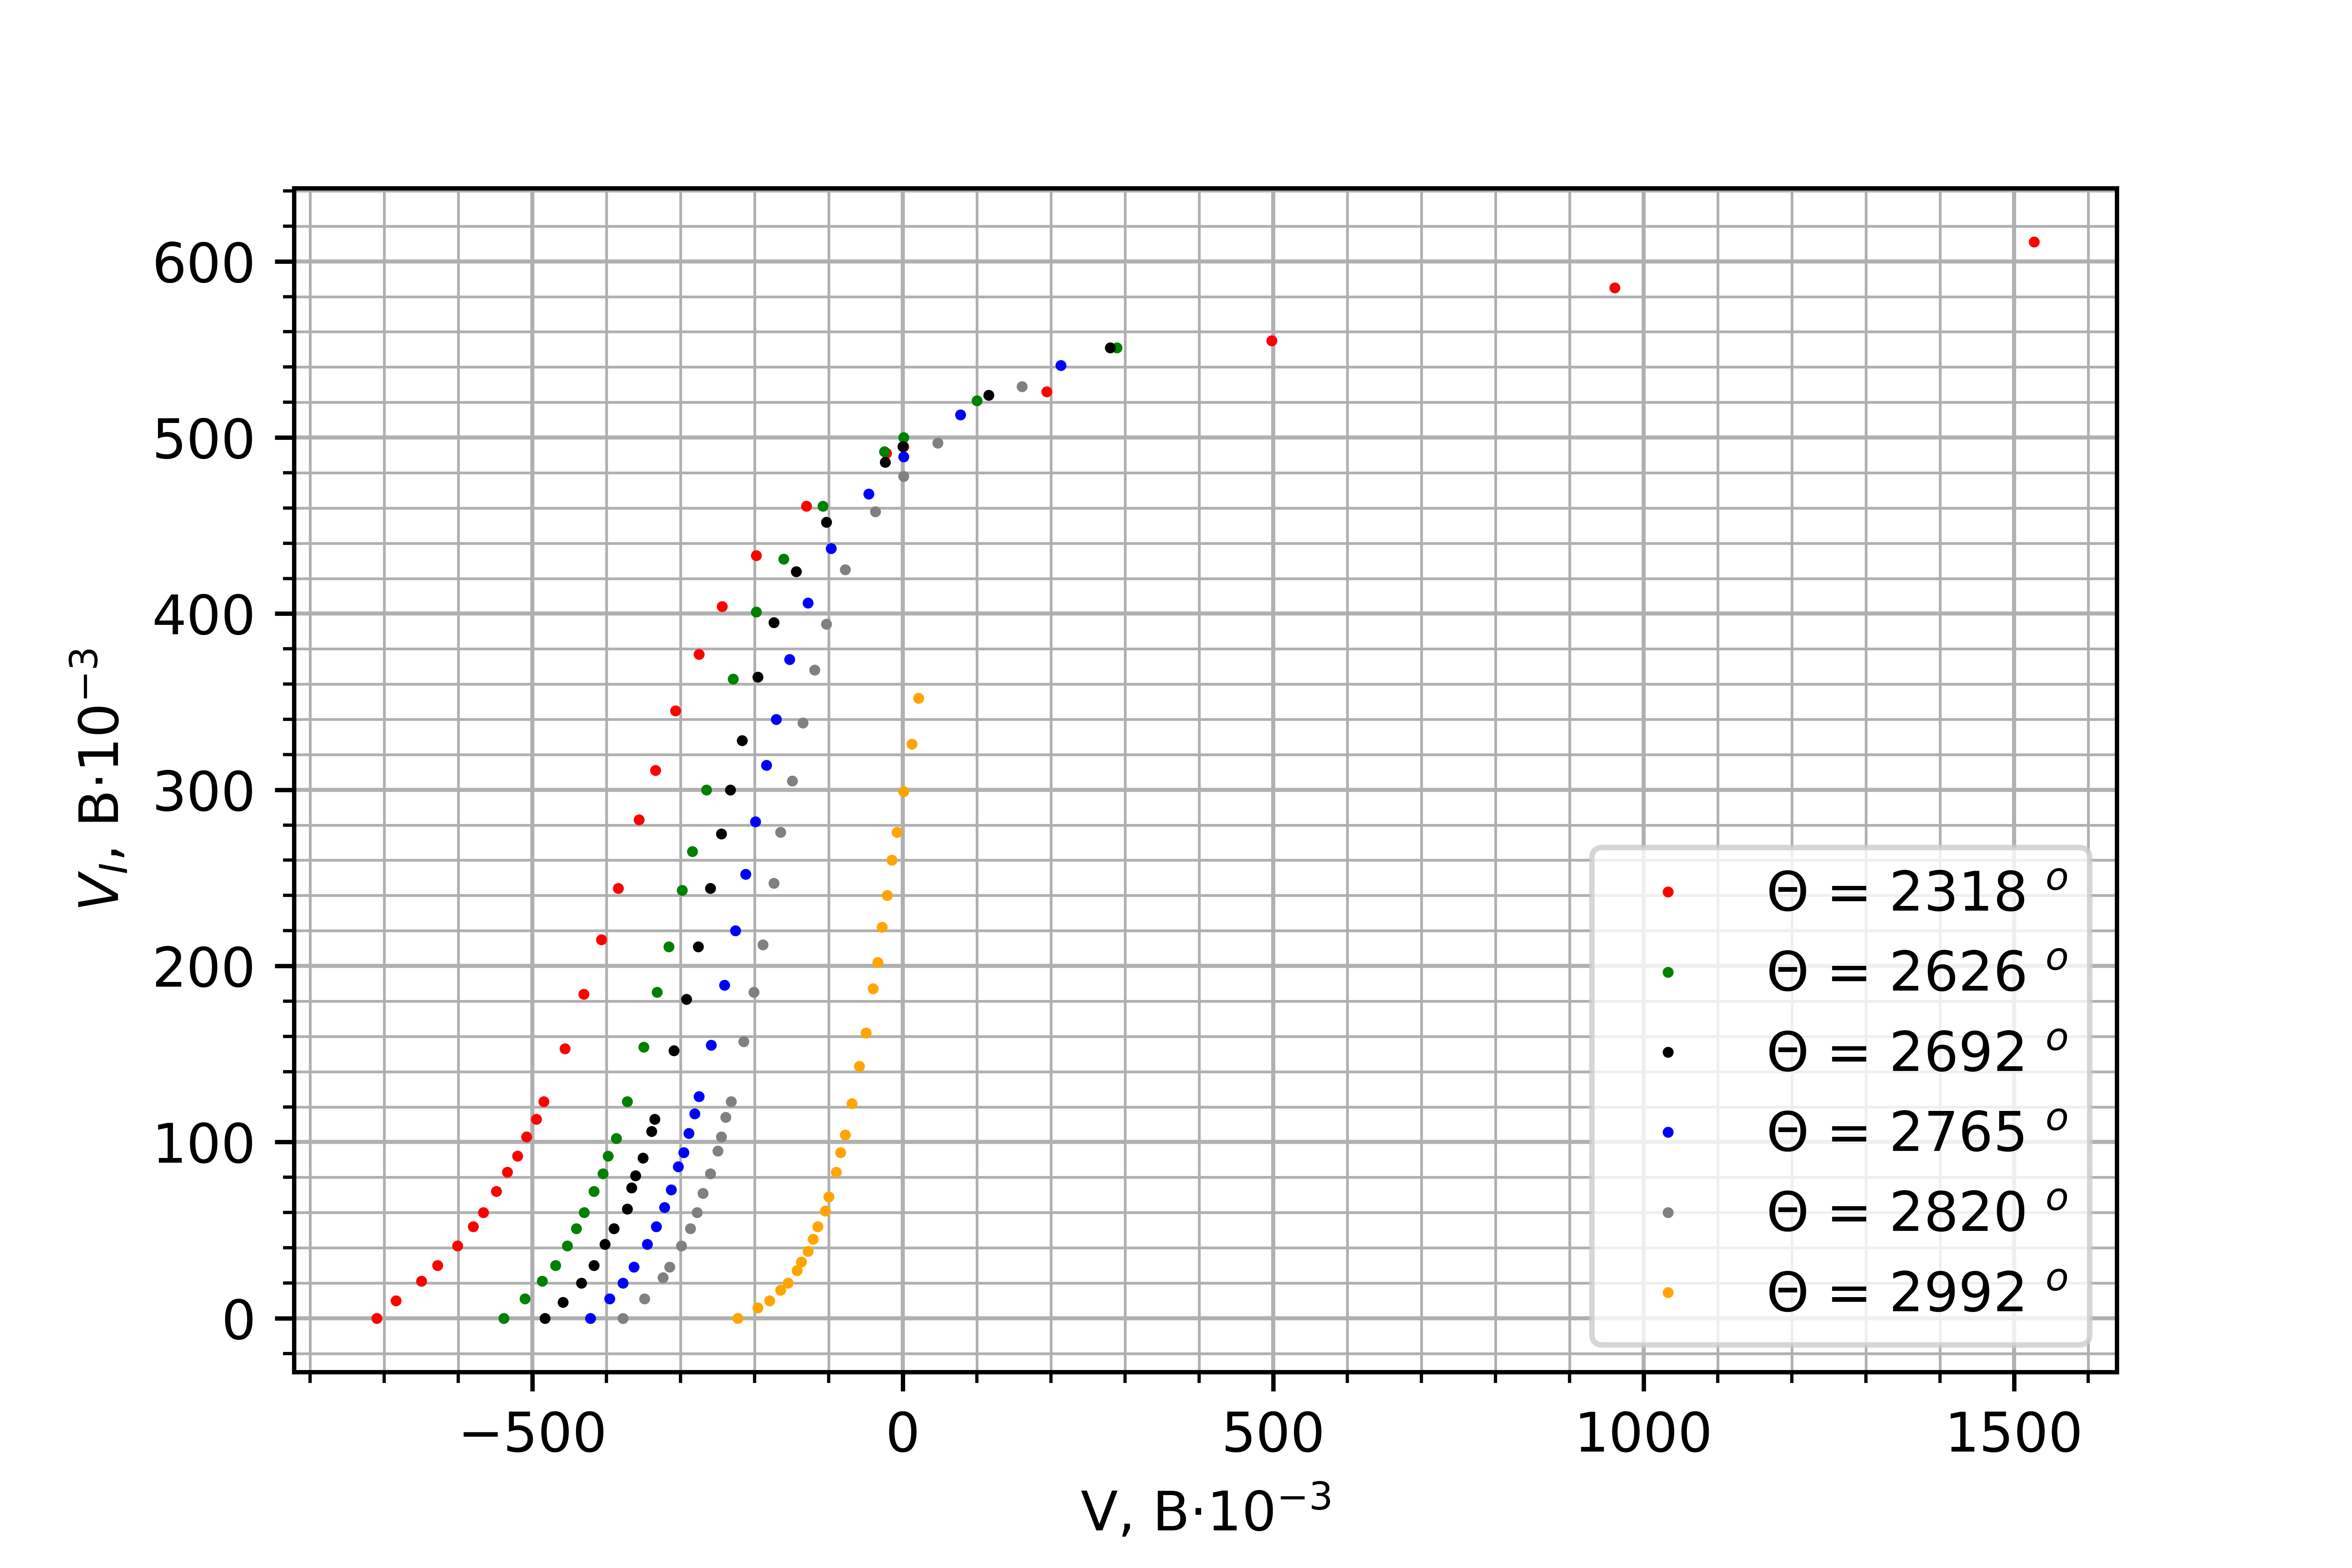
\includegraphics[width=0.7\linewidth]{V_I(V).png}
		\caption{Зависимость $V_{I}(V)$}
	\end{figure}
Построив зависимость $\sqrt{V_{I}}(V)$ для параболической части графика(см.рис. \ref{ris grad}), найдем запирающий потенциал для разных длин волн:

	\begin{figure}[H]
		\centering
		\includegraphics[width=0.7\linewidth]{sqrt{V_I}(V).png}
		\caption{Зависимость $\sqrt{V_{I}}(V)$}
	\end{figure}

Получим зависимость запирающего потенциала от частоты падающего света:

\begin{table}[H]
\begin{tabular}{|c|c|c|}
\hline
$V_{0},$ В$\cdot 10^{-3}$  & $\omega, c^{-1} \cdot 10^{15}$ & $\sigma_{\omega}, c^{-1} \cdot 10^{15}$ \\ \hline
750 & 3,489 & 0,016       \\ \hline
565 & 3,168 & 0,013       \\ \hline
502 & 3,093 & 0,012       \\ \hline
439 & 3,007 & 0,011       \\ \hline
387 & 2,939 & 0,011       \\ \hline
211 & 2,719 & 0,010       \\ \hline
\end{tabular}
\caption{Зависимость $V_{0}(\omega)$}
\end{table}

Построим соответствующий график:

	\begin{figure}[H]
		\centering
		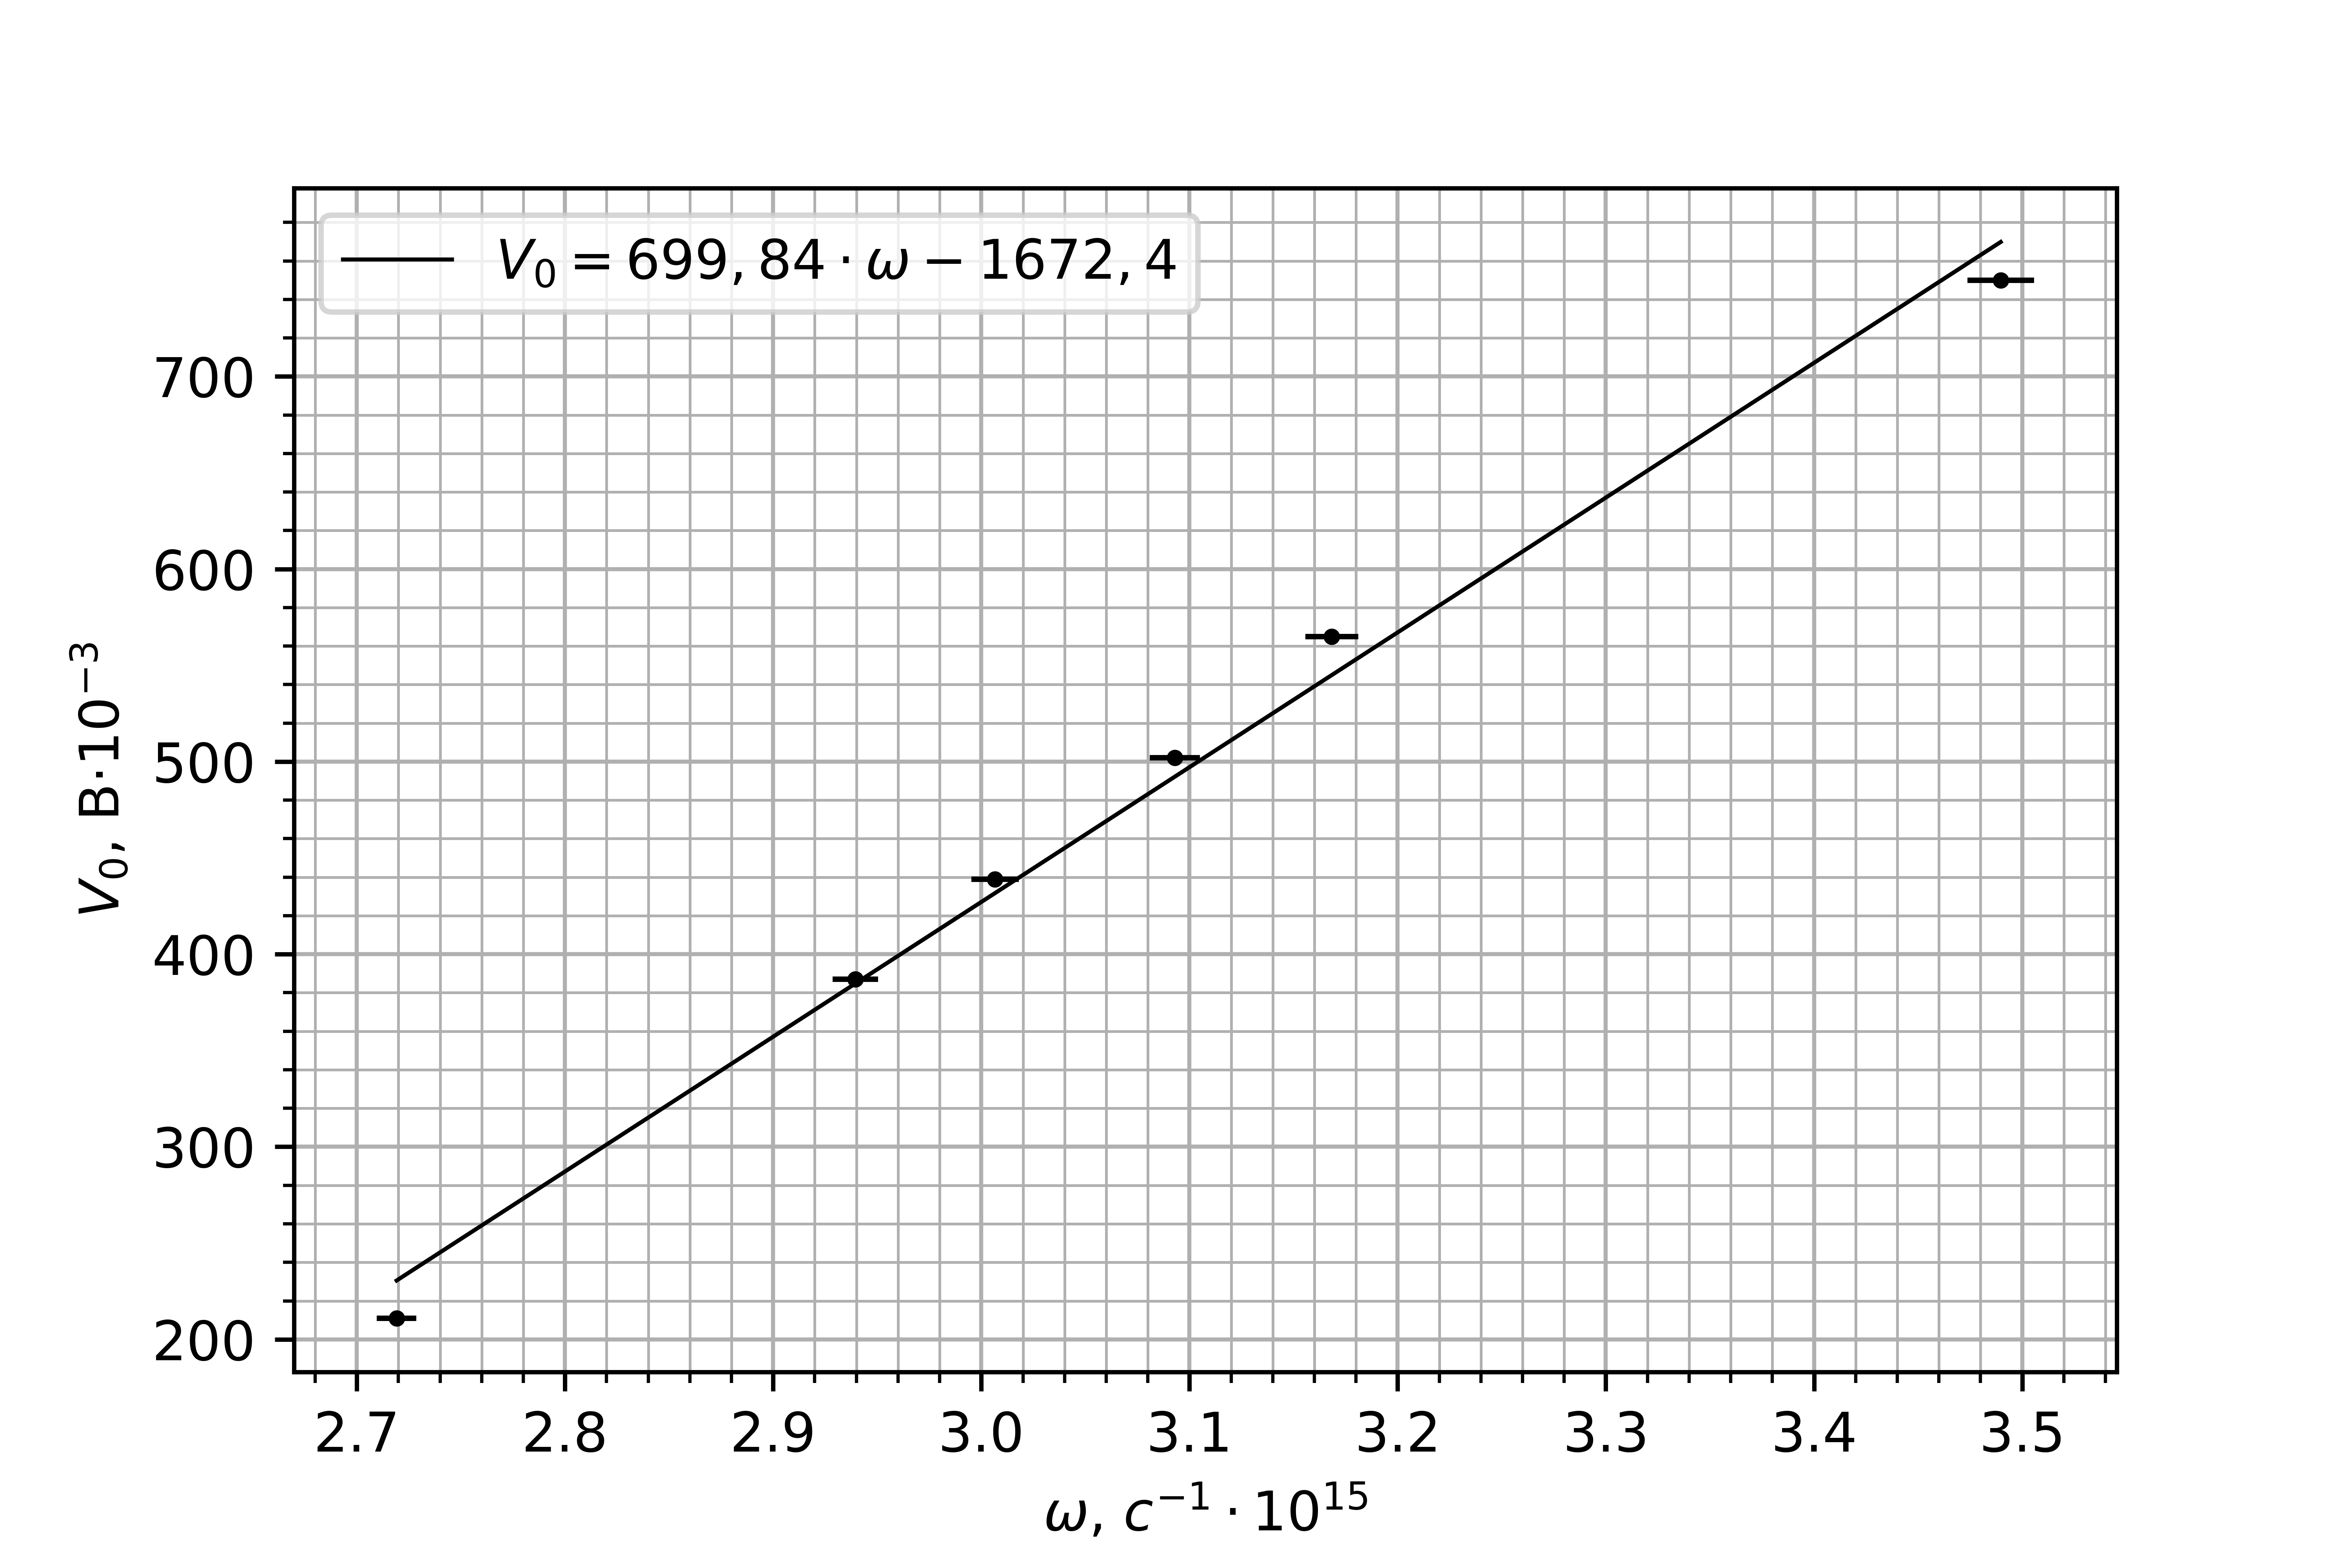
\includegraphics[width=0.7\linewidth]{V_0(omega).png}
		\caption{Зависимость $\sqrt{V_{I}}(V)$}
	\end{figure}

По наклону графика можем найти постоянную Планка по формуле:

\begin{equation*}
    \hbar = \frac{dV_{0}}{d\omega}\cdot e = (1,12 \pm 0,13)\cdot 10^{-34} \text{Дж}\cdot\text{с}
\end{equation*}

Погрешность постоянной Планка считалась по формуле:

\begin{equation*}
    \sigma_{\hbar} = \sigma_{\frac{dV_{0}}{d\omega}}\cdot e,
\end{equation*}

где $\sigma_{\frac{dV_{0}}{d\omega}}$ была найдена из МНК

Отметим, что полученное значение сходится с теоретическим ($\hbar = 1,054 \cdot 10^{-34} \text{Дж}\cdot\text{с}$) в пределах $\sigma$.

\section*{5. Выводы}
В данной работе мы убедились в справедливости описания Эйнштейна для фотоэффекта. Также были найдены запирающие потенциалы для 6 длин волн. Построена зависимость запирающего потенциала от частоты падающего излучения, откуда мы получили экспериментальное значение величины постоянной Планка, которая в пределах $\sigma$ сходится с теоретическим.
	
\section*{6. Приложение}
\begin{table}[H]
\begin{tabular}{|c|c|c|c|c|c|}
\hline
$V_{I}$,В$\cdot10^{-3}$ & $\sigma_{V_I}$,В$\cdot10^{-3}$ & $\sqrt_{V_I}$,В$\cdot10^{-3}$ & $\sigma_{\sqrt_{V_I}}$,В$\cdot10^{-3}$ & $V$,В$\cdot10^{-3}$ & $\sigma_{V}$,В$\cdot10^{-3}$ \\ \hline
0                             & \multirow{15}{*}{1}                   & 0,00                              & -                                 & -710                         & \multirow{15}{*}{1}                  \\ \cline{1-1} \cline{3-5}
10                            &                                       & 3,16                              & 0,16                              & -684                         &                                      \\ \cline{1-1} \cline{3-5}
21                            &                                       & 4,58                              & 0,11                              & -650                         &                                      \\ \cline{1-1} \cline{3-5}
30                            &                                       & 5,48                              & 0,09                              & -628                         &                                      \\ \cline{1-1} \cline{3-5}
41                            &                                       & 6,40                              & 0,08                              & -601                         &                                      \\ \cline{1-1} \cline{3-5}
52                            &                                       & 7,21                              & 0,07                              & -580                         &                                      \\ \cline{1-1} \cline{3-5}
60                            &                                       & 7,75                              & 0,06                              & -566                         &                                      \\ \cline{1-1} \cline{3-5}
72                            &                                       & 8,49                              & 0,06                              & -549                         &                                      \\ \cline{1-1} \cline{3-5}
83                            &                                       & 9,11                              & 0,05                              & -534                         &                                      \\ \cline{1-1} \cline{3-5}
92                            &                                       & 9,59                              & 0,05                              & -520                         &                                      \\ \cline{1-1} \cline{3-5}
103                           &                                       & 10,15                             & 0,05                              & -508                         &                                      \\ \cline{1-1} \cline{3-5}
113                           &                                       & 10,63                             & 0,05                              & -495                         &                                      \\ \cline{1-1} \cline{3-5}
123                           &                                       & 11,09                             & 0,05                              & -485                         &                                      \\ \cline{1-1} \cline{3-5}
153                           &                                       & 12,37                             & 0,04                              & -456                         &                                      \\ \cline{1-1} \cline{3-5}
184                           &                                       & 13,56                             & 0,04                              & -431                         &                                      \\ \hline
215 & \multirow{15}{*}{1} & 14,66 & 0,03 & -407 & \multirow{15}{*}{1} \\ \cline{1-1} \cline{3-5}
244 &                     & 15,62 & 0,03 & -384 &                     \\ \cline{1-1} \cline{3-5}
283 &                     & 16,82 & 0,03 & -356 &                     \\ \cline{1-1} \cline{3-5}
311 &                     & 17,64 & 0,03 & -334 &                     \\ \cline{1-1} \cline{3-5}
345 &                     & 18,57 & 0,03 & -307 &                     \\ \cline{1-1} \cline{3-5}
377 &                     & 19,42 & 0,03 & -275 &                     \\ \cline{1-1} \cline{3-5}
404 &                     & 20,10 & 0,02 & -244 &                     \\ \cline{1-1} \cline{3-5}
433 &                     & 20,81 & 0,02 & -198 &                     \\ \cline{1-1} \cline{3-5}
461 &                     & 21,47 & 0,02 & -130 &                     \\ \cline{1-1} \cline{3-5}
491 &                     & 22,16 & 0,02 & -22  &                     \\ \cline{1-1} \cline{3-5}
495 &                     & 22,25 & 0,02 & 1    &                     \\ \cline{1-1} \cline{3-5}
526 &                     & 22,93 & 0,02 & 194  &                     \\ \cline{1-1} \cline{3-5}
555 &                     & 23,56 & 0,02 & 498  &                     \\ \cline{1-1} \cline{3-5}
585 &                     & 24,19 & 0,02 & 961  &                     \\ \cline{1-1} \cline{3-5}
611 &                     & 24,72 & 0,02 & 1527 &                     \\ \hline
\end{tabular}
\caption{Измерение для $\Theta = (2318\pm 1) ^{o}$}
\end{table}

\begin{table}[H]
\begin{tabular}{|c|c|c|c|c|c|}
\hline
$V_{I}$,В$\cdot10^{-3}$ & $\sigma_{V_I}$,В$\cdot10^{-3}$ & $\sqrt_{V_I}$,В$\cdot10^{-3}$ & $\sigma_{\sqrt_{V_I}}$,В$\cdot10^{-3}$ & $V$,В$\cdot10^{-3}$ & $\sigma_{V}$,В$\cdot10^{-3}$ \\ \hline
0                             & \multirow{13}{*}{1}                   & 0,00                              & -                                 & -539                         & \multirow{13}{*}{1}                  \\ \cline{1-1} \cline{3-5}
11                            &                                       & 3,32                              & 0,15                              & -510                         &                                      \\ \cline{1-1} \cline{3-5}
21                            &                                       & 4,58                              & 0,11                              & -487                         &                                      \\ \cline{1-1} \cline{3-5}
30                            &                                       & 5,48                              & 0,09                              & -469                         &                                      \\ \cline{1-1} \cline{3-5}
41                            &                                       & 6,40                              & 0,08                              & -453                         &                                      \\ \cline{1-1} \cline{3-5}
51                            &                                       & 7,14                              & 0,07                              & -441                         &                                      \\ \cline{1-1} \cline{3-5}
60                            &                                       & 7,75                              & 0,06                              & -430                         &                                      \\ \cline{1-1} \cline{3-5}
72                            &                                       & 8,49                              & 0,06                              & -417                         &                                      \\ \cline{1-1} \cline{3-5}
82                            &                                       & 9,06                              & 0,06                              & -405                         &                                      \\ \cline{1-1} \cline{3-5}
92                            &                                       & 9,59                              & 0,05                              & -398                         &                                      \\ \cline{1-1} \cline{3-5}
102                           &                                       & 10,10                             & 0,05                              & -387                         &                                      \\ \cline{1-1} \cline{3-5}
123                           &                                       & 11,09                             & 0,05                              & -372                         &                                      \\ \cline{1-1} \cline{3-5}
154                           &                                       & 12,41                             & 0,04                              & -350                         &                                      \\ \hline
185 & \multirow{13}{*}{1} & 13,60 & 0,04 & -332 & \multirow{13}{*}{1} \\ \cline{1-1} \cline{3-5}
211 &                     & 14,53 & 0,03 & -316 &                     \\ \cline{1-1} \cline{3-5}
243 &                     & 15,59 & 0,03 & -298 &                     \\ \cline{1-1} \cline{3-5}
265 &                     & 16,28 & 0,03 & -284 &                     \\ \cline{1-1} \cline{3-5}
300 &                     & 17,32 & 0,03 & -265 &                     \\ \cline{1-1} \cline{3-5}
363 &                     & 19,05 & 0,03 & -229 &                     \\ \cline{1-1} \cline{3-5}
401 &                     & 20,02 & 0,02 & -198 &                     \\ \cline{1-1} \cline{3-5}
431 &                     & 20,76 & 0,02 & -161 &                     \\ \cline{1-1} \cline{3-5}
461 &                     & 21,47 & 0,02 & -108 &                     \\ \cline{1-1} \cline{3-5}
492 &                     & 22,18 & 0,02 & -25  &                     \\ \cline{1-1} \cline{3-5}
500 &                     & 22,36 & 0,02 & 1    &                     \\ \cline{1-1} \cline{3-5}
521 &                     & 22,83 & 0,02 & 100  &                     \\ \cline{1-1} \cline{3-5}
551 &                     & 23,47 & 0,02 & 289  &                     \\ \hline
\end{tabular}
\caption{Измерение для $\Theta = (2626\pm 1) ^{o}$}
\end{table}

\begin{table}[H]
\begin{tabular}{|c|c|c|c|c|c|}
\hline
$V_{I}$,В$\cdot10^{-3}$ & $\sigma_{V_I}$,В$\cdot10^{-3}$ & $\sqrt_{V_I}$,В$\cdot10^{-3}$ & $\sigma_{\sqrt_{V_I}}$,В$\cdot10^{-3}$ & $V$,В$\cdot10^{-3}$ & $\sigma_{V}$,В$\cdot10^{-3}$  \\ \hline
0                             & \multirow{14}{*}{1}                   & 0,00                              & -                                 & -483                         & \multirow{14}{*}{1}                  \\ \cline{1-1} \cline{3-5}
9                             &                                       & 3,00                              & 0,17                              & -459                         &                                      \\ \cline{1-1} \cline{3-5}
20                            &                                       & 4,47                              & 0,11                              & -434                         &                                      \\ \cline{1-1} \cline{3-5}
30                            &                                       & 5,48                              & 0,09                              & -417                         &                                      \\ \cline{1-1} \cline{3-5}
42                            &                                       & 6,48                              & 0,08                              & -402                         &                                      \\ \cline{1-1} \cline{3-5}
51                            &                                       & 7,14                              & 0,07                              & -390                         &                                      \\ \cline{1-1} \cline{3-5}
62                            &                                       & 7,87                              & 0,06                              & -372                         &                                      \\ \cline{1-1} \cline{3-5}
74                            &                                       & 8,60                              & 0,06                              & -366                         &                                      \\ \cline{1-1} \cline{3-5}
81                            &                                       & 9,00                              & 0,06                              & -361                         &                                      \\ \cline{1-1} \cline{3-5}
91                            &                                       & 9,54                              & 0,05                              & -351                         &                                      \\ \cline{1-1} \cline{3-5}
106                           &                                       & 10,30                             & 0,05                              & -339                         &                                      \\ \cline{1-1} \cline{3-5}
113                           &                                       & 10,63                             & 0,05                              & -335                         &                                      \\ \cline{1-1} \cline{3-5}
152                           &                                       & 12,33                             & 0,04                              & -309                         &                                      \\ \cline{1-1} \cline{3-5}
181                           &                                       & 13,45                             & 0,04                              & -292                         &                                      \\ \hline
211 & \multirow{13}{*}{1} & 14,53 & 0,03 & -276 & \multirow{13}{*}{1} \\ \cline{1-1} \cline{3-5}
244 &                     & 15,62 & 0,03 & -260 &                     \\ \cline{1-1} \cline{3-5}
275 &                     & 16,58 & 0,03 & -245 &                     \\ \cline{1-1} \cline{3-5}
300 &                     & 17,32 & 0,03 & -233 &                     \\ \cline{1-1} \cline{3-5}
328 &                     & 18,11 & 0,03 & -217 &                     \\ \cline{1-1} \cline{3-5}
364 &                     & 19,08 & 0,03 & -196 &                     \\ \cline{1-1} \cline{3-5}
395 &                     & 19,87 & 0,03 & -174 &                     \\ \cline{1-1} \cline{3-5}
424 &                     & 20,59 & 0,02 & -144 &                     \\ \cline{1-1} \cline{3-5}
452 &                     & 21,26 & 0,02 & -103 &                     \\ \cline{1-1} \cline{3-5}
486 &                     & 22,05 & 0,02 & -24  &                     \\ \cline{1-1} \cline{3-5}
495 &                     & 22,25 & 0,02 & 0    &                     \\ \cline{1-1} \cline{3-5}
524 &                     & 22,89 & 0,02 & 116  &                     \\ \cline{1-1} \cline{3-5}
551 &                     & 23,47 & 0,02 & 280  &                     \\ \hline
\end{tabular}
\caption{Измерение для $\Theta = (2692\pm 1) ^{o}$}
\end{table}

\begin{table}[H]
\begin{tabular}{|c|c|c|c|c|c|}
\hline
$V_{I}$,В$\cdot10^{-3}$ & $\sigma_{V_I}$,В$\cdot10^{-3}$ & $\sqrt_{V_I}$,В$\cdot10^{-3}$ & $\sigma_{\sqrt_{V_I}}$,В$\cdot10^{-3}$ & $V$,В$\cdot10^{-3}$ & $\sigma_{V}$,В$\cdot10^{-3}$ \\ \hline
0                             & \multirow{14}{*}{1}                   & 0,00                              & -                                 & -422                         & \multirow{14}{*}{1}                  \\ \cline{1-1} \cline{3-5}
11                            &                                       & 3,32                              & 0,15                              & -396                         &                                      \\ \cline{1-1} \cline{3-5}
20                            &                                       & 4,47                              & 0,11                              & -378                         &                                      \\ \cline{1-1} \cline{3-5}
29                            &                                       & 5,39                              & 0,09                              & -363                         &                                      \\ \cline{1-1} \cline{3-5}
42                            &                                       & 6,48                              & 0,08                              & -345                         &                                      \\ \cline{1-1} \cline{3-5}
52                            &                                       & 7,21                              & 0,07                              & -333                         &                                      \\ \cline{1-1} \cline{3-5}
63                            &                                       & 7,94                              & 0,06                              & -322                         &                                      \\ \cline{1-1} \cline{3-5}
73                            &                                       & 8,54                              & 0,06                              & -313                         &                                      \\ \cline{1-1} \cline{3-5}
86                            &                                       & 9,27                              & 0,05                              & -303                         &                                      \\ \cline{1-1} \cline{3-5}
94                            &                                       & 9,70                              & 0,05                              & -296                         &                                      \\ \cline{1-1} \cline{3-5}
105                           &                                       & 10,25                             & 0,05                              & -289                         &                                      \\ \cline{1-1} \cline{3-5}
116                           &                                       & 10,77                             & 0,05                              & -281                         &                                      \\ \cline{1-1} \cline{3-5}
126                           &                                       & 11,22                             & 0,04                              & -275                         &                                      \\ \cline{1-1} \cline{3-5}
155                           &                                       & 12,45                             & 0,04                              & -259                         &                                      \\ \hline
189 & \multirow{13}{*}{1} & 13,75 & 0,04 & -241 & \multirow{13}{*}{1} \\ \cline{1-1} \cline{3-5}
220 &                     & 14,83 & 0,03 & -226 &                     \\ \cline{1-1} \cline{3-5}
252 &                     & 15,87 & 0,03 & -212 &                     \\ \cline{1-1} \cline{3-5}
282 &                     & 16,79 & 0,03 & -199 &                     \\ \cline{1-1} \cline{3-5}
314 &                     & 17,72 & 0,03 & -184 &                     \\ \cline{1-1} \cline{3-5}
340 &                     & 18,44 & 0,03 & -171 &                     \\ \cline{1-1} \cline{3-5}
374 &                     & 19,34 & 0,03 & -153 &                     \\ \cline{1-1} \cline{3-5}
406 &                     & 20,15 & 0,02 & -128 &                     \\ \cline{1-1} \cline{3-5}
437 &                     & 20,90 & 0,02 & -97  &                     \\ \cline{1-1} \cline{3-5}
468 &                     & 21,63 & 0,02 & -46  &                     \\ \cline{1-1} \cline{3-5}
489 &                     & 22,11 & 0,02 & 1    &                     \\ \cline{1-1} \cline{3-5}
513 &                     & 22,65 & 0,02 & 78   &                     \\ \cline{1-1} \cline{3-5}
541 &                     & 23,26 & 0,02 & 213  &                     \\ \hline
\end{tabular}
\caption{Измерение для $\Theta = (2765\pm 1) ^{o}$}
\end{table}

\begin{table}[H]
\begin{tabular}{|c|c|c|c|c|c|}
\hline
$V_{I}$,В$\cdot10^{-3}$ & $\sigma_{V_I}$,В$\cdot10^{-3}$ & $\sqrt_{V_I}$,В$\cdot10^{-3}$ & $\sigma_{\sqrt_{V_I}}$,В$\cdot10^{-3}$ & $V$,В$\cdot10^{-3}$ & $\sigma_{V}$,В$\cdot10^{-3}$ \\ \hline
0                             & \multirow{14}{*}{1}                   & 0,00                              & -                                 & -378                         & \multirow{14}{*}{1}                  \\ \cline{1-1} \cline{3-5}
11                            &                                       & 3,32                              & 0,15                              & -349                         &                                      \\ \cline{1-1} \cline{3-5}
23                            &                                       & 4,80                              & 0,10                              & -324                         &                                      \\ \cline{1-1} \cline{3-5}
29                            &                                       & 5,39                              & 0,09                              & -315                         &                                      \\ \cline{1-1} \cline{3-5}
41                            &                                       & 6,40                              & 0,08                              & -299                         &                                      \\ \cline{1-1} \cline{3-5}
51                            &                                       & 7,14                              & 0,07                              & -287                         &                                      \\ \cline{1-1} \cline{3-5}
60                            &                                       & 7,75                              & 0,06                              & -278                         &                                      \\ \cline{1-1} \cline{3-5}
71                            &                                       & 8,43                              & 0,06                              & -270                         &                                      \\ \cline{1-1} \cline{3-5}
82                            &                                       & 9,06                              & 0,06                              & -260                         &                                      \\ \cline{1-1} \cline{3-5}
95                            &                                       & 9,75                              & 0,05                              & -250                         &                                      \\ \cline{1-1} \cline{3-5}
103                           &                                       & 10,15                             & 0,05                              & -245                         &                                      \\ \cline{1-1} \cline{3-5}
114                           &                                       & 10,68                             & 0,05                              & -239                         &                                      \\ \cline{1-1} \cline{3-5}
123                           &                                       & 11,09                             & 0,05                              & -232                         &                                      \\ \cline{1-1} \cline{3-5}
157                           &                                       & 12,53                             & 0,04                              & -215                         &                                      \\ \hline
185 & \multirow{13}{*}{1} & 13,60 & 0,04 & -201 & \multirow{13}{*}{1} \\ \cline{1-1} \cline{3-5}
212 &                     & 14,56 & 0,03 & -189 &                     \\ \cline{1-1} \cline{3-5}
247 &                     & 15,72 & 0,03 & -174 &                     \\ \cline{1-1} \cline{3-5}
276 &                     & 16,61 & 0,03 & -165 &                     \\ \cline{1-1} \cline{3-5}
305 &                     & 17,46 & 0,03 & -149 &                     \\ \cline{1-1} \cline{3-5}
338 &                     & 18,38 & 0,03 & -135 &                     \\ \cline{1-1} \cline{3-5}
368 &                     & 19,18 & 0,03 & -119 &                     \\ \cline{1-1} \cline{3-5}
394 &                     & 19,85 & 0,03 & -103 &                     \\ \cline{1-1} \cline{3-5}
425 &                     & 20,62 & 0,02 & -78  &                     \\ \cline{1-1} \cline{3-5}
458 &                     & 21,40 & 0,02 & -37  &                     \\ \cline{1-1} \cline{3-5}
478 &                     & 21,86 & 0,02 & 1    &                     \\ \cline{1-1} \cline{3-5}
497 &                     & 22,29 & 0,02 & 47   &                     \\ \cline{1-1} \cline{3-5}
529 &                     & 23,00 & 0,02 & 161  &                     \\ \hline
\end{tabular}
\caption{Измерение для $\Theta = (2820\pm 1) ^{o}$}
\end{table}

\begin{table}[H]
\begin{tabular}{|c|c|c|c|c|c|}
\hline
$V_{I}$,В$\cdot10^{-3}$ & $\sigma_{V_I}$,В$\cdot10^{-3}$ & $\sqrt_{V_I}$,В$\cdot10^{-3}$ & $\sigma_{\sqrt_{V_I}}$,В$\cdot10^{-3}$ & $V$,В$\cdot10^{-3}$ & $\sigma_{V}$,В$\cdot10^{-3}$ \\ \hline
0                             & \multirow{14}{*}{1}                   & 0,00                              & -                                 & -223                         & \multirow{14}{*}{1}                  \\ \cline{1-1} \cline{3-5}
6                             &                                       & 2,45                              & 0,20                              & -196                         &                                      \\ \cline{1-1} \cline{3-5}
10                            &                                       & 3,16                              & 0,16                              & -180                         &                                      \\ \cline{1-1} \cline{3-5}
16                            &                                       & 4,00                              & 0,13                              & -165                         &                                      \\ \cline{1-1} \cline{3-5}
20                            &                                       & 4,47                              & 0,11                              & -155                         &                                      \\ \cline{1-1} \cline{3-5}
27                            &                                       & 5,20                              & 0,10                              & -143                         &                                      \\ \cline{1-1} \cline{3-5}
32                            &                                       & 5,66                              & 0,09                              & -137                         &                                      \\ \cline{1-1} \cline{3-5}
38                            &                                       & 6,16                              & 0,08                              & -128                         &                                      \\ \cline{1-1} \cline{3-5}
45                            &                                       & 6,71                              & 0,07                              & -121                         &                                      \\ \cline{1-1} \cline{3-5}
52                            &                                       & 7,21                              & 0,07                              & -115                         &                                      \\ \cline{1-1} \cline{3-5}
61                            &                                       & 7,81                              & 0,06                              & -105                         &                                      \\ \cline{1-1} \cline{3-5}
69                            &                                       & 8,31                              & 0,06                              & -100                         &                                      \\ \cline{1-1} \cline{3-5}
83                            &                                       & 9,11                              & 0,05                              & -90                          &                                      \\ \cline{1-1} \cline{3-5}
94                            &                                       & 9,70                              & 0,05                              & -84                          &                                      \\ \hline
104 & \multirow{13}{*}{1} & 10,20 & 0,05 & -78 & \multirow{13}{*}{1} \\ \cline{1-1} \cline{3-5}
122 &                     & 11,05 & 0,05 & -69 &                     \\ \cline{1-1} \cline{3-5}
143 &                     & 11,96 & 0,04 & -59 &                     \\ \cline{1-1} \cline{3-5}
162 &                     & 12,73 & 0,04 & -50 &                     \\ \cline{1-1} \cline{3-5}
187 &                     & 13,67 & 0,04 & -40 &                     \\ \cline{1-1} \cline{3-5}
202 &                     & 14,21 & 0,04 & -34 &                     \\ \cline{1-1} \cline{3-5}
222 &                     & 14,90 & 0,03 & -28 &                     \\ \cline{1-1} \cline{3-5}
240 &                     & 15,49 & 0,03 & -21 &                     \\ \cline{1-1} \cline{3-5}
260 &                     & 16,12 & 0,03 & -15 &                     \\ \cline{1-1} \cline{3-5}
276 &                     & 16,61 & 0,03 & -8  &                     \\ \cline{1-1} \cline{3-5}
299 &                     & 17,29 & 0,03 & 1   &                     \\ \cline{1-1} \cline{3-5}
326 &                     & 18,06 & 0,03 & 12  &                     \\ \cline{1-1} \cline{3-5}
352 &                     & 18,76 & 0,03 & 21  &                     \\ \hline
\end{tabular}
\caption{Измерение для $\Theta = (2992\pm 1) ^{o}$}
\end{table}

\end{document}
